%%%%%%%%%%%%%%%%%%%%%%%%%%%%%%%%%%%%%%%%%%%%%%%%%%%%%%%%%%%%%%%%%%%%%%%%%%%%%%%%
%2345678901234567890123456789012345678901234567890123456789012345678901234567890
%        1         2         3         4         5         6         7         8

\documentclass[letterpaper, 10 pt, conference]{ieeeconf}  % Comment this line out if you need a4paper
\usepackage[colorlinks,linkcolor=black]{hyperref}

%\documentclass[a4paper, 10pt, conference]{ieeeconf}      % Use this line for a4 paper

\IEEEoverridecommandlockouts                              % This command is only needed if
                                                          % you want to use the \thanks command

\overrideIEEEmargins                                      % Needed to meet printer requirements.

%In case you encounter the following error:
%Error 1010 The PDF file may be corrupt (unable to open PDF file) OR
%Error 1000 An error occurred while parsing a contents stream. Unable to analyze the PDF file.
%This is a known problem with pdfLaTeX conversion filter. The file cannot be opened with acrobat reader
%Please use one of the alternatives below to circumvent this error by uncommenting one or the other
%\pdfobjcompresslevel=0
%\pdfminorversion=4

% See the \addtolength command later in the file to balance the column lengths
% on the last page of the document

% The following packages can be found on http:\\www.ctan.org
\usepackage{amsmath} % assumes amsmath package installed
\usepackage{amssymb}  % assumes amsmath package installed

\usepackage{amsfonts}
\usepackage{cite}
%\usepackage{algorithmic}
\usepackage{graphicx}
\usepackage{subcaption}% needed for subfigure
\usepackage{diagbox}
%\usepackage{biblatex}
%\usepackage{textcomp}
\usepackage{xargs}
\usepackage[pdftex,dvipsnames,table]{xcolor}
\usepackage{dirtree}
\usepackage{multirow}
\usepackage{verbatim}
\title{\LARGE \bf
SUSTech POINTS: An Efficient 3D Point Cloud Annotation Platform
}

\author{E Li$^{1}$,Shuaijun Wang$^{1,2}$,  Chengyang Li$^{1}$, Dachuan Li$^{1}$,Xiangbin Wu$^{3}$, and Qi Hao$^{1,*}$% <-this % stops a space
\thanks{This work is partially supported by the National Natural Science Foundation of China (No: 61773197), the Science and Technology Innovation Committee of Shenzhen City (No: GJHZ20170314114424152), the Nanshan District Science and Technology Innovation Bureau (No: LHTD20170007), and the Intel ICRI-IACV Research Fund (CG$\#$52514373).}
\thanks{$^{*}$Corresponding author: Qi Hao (hao.q@sustech.edu.cn).}
\thanks{$^{1}$Department of Computer Science and Engineering,
Southern University of Science and Technology, Shenzhen, Guangdong, China, 518055}
\thanks{$^{2}$Harbin Institute of Technology,
92 West Dazhi Street, Nan Gang District, Harbin, China, 150001}%
% <-this % stops a space
\thanks{$^{3}$ Intel Corporation}%
% <-this % stops a space
}


\begin{document}
\maketitle
\thispagestyle{empty}
\pagestyle{empty}
%%%%%%%%%%%%%%%%%%%%%%%%%%%%%%%%%%%%%%%%%%%%%%%%%%%%%%%%%%%%%%%%%%%%%%%%%%%%%%%%
\begin{abstract}


The major challenges of developing 3D object annotation platforms for autonomous driving datasets 
include efficient operations on geometric data units, convenient user interfaces and scalable annotation tools, This paper presents a novel annotation platform (i.e. SUSTech POINTS), which contains a set of efficient annotation tools (operations) and user-friendly interfaces to help achieve high-quality data annotations with high efficiency.
The novelty of this work includes threefolds: 
(1) developing a set of visulization functionalities for convenient user-data interactions;
(2) developing a set of efficient operations for labelling 3D point clouds and 2D images; 
(3) developing a transfer annotation method to label the same objects in related frames. 
The developed platform is tested with the KITTI, nuScenes, and a self-collected dataset. 
The experimental results show that the developed platform can improve the annotation efficiency and accuracy pretty much 
compared with using other open-source platforms.
\end{abstract}


%%%%%%%%%%%%%%%%%%%%%%%%%%%%%%%%%%%%%%%%%%%%%%%%%%%%%%%%%%%%%%%%%%%%%%%%%%%%%%%%




\section{INTRODUCTION}


Building accurately annotated autonomous driving datasets is critical for training and verification of various perception and data fusion algorithms. There are three major components for antonomous driving dataset annotations: (1) data pre-processing, (2) data visualizations, and (3) manual operations, which are enabled by a data management system and a user interaction platform, as shown in Fig. 1. In the data pre-processing, intrinsic/extrinsic sensor parameters are estimated first; only those data frames consistent to calibration parameters, useful for algorithms training and verification are selected; then a set of algorithms including detection, segmentation, and 2D/3d fusion are used to annotate the dataset initially. The data visualizations usually provide helpful spatial/temporal navigation tools for users, distinguish data of different objects, and show multiple views of each object from different perspectives. The most useful manual data operations include labels editing in multiple views, automatically adjusting the size of 2D/3D boxes to fit the data of one object, and automatically extending annotations of the same objects to different frames (modalities).



Despite efforts and successes in developing AI-based pre-processing techniques, data visualizations and manual operations also impose various technical challenges for developing an efficient data annotation platform, including
\begin{enumerate}
	\item Fast Error Checking.  Given those 2D and 3D multiple perspectives data frames, it is necessary to guarantee their consistency with each other in a high speed.
	\item Easy human-data interactions. Each frame of data usually contains a great number of objects with irregular measurement data in a large field of view, hence it is necessary to develop an convenient human-computer interface to enable users to check data annotations and perform corresponding operations.
	\item Flexible annotation extension. There are a lot correlations among data frames, observation areas, and sensing modalities, so the annotations of the same objects should be scalable and extensible among different frames, areas and modalities.
\end{enumerate}

\begin{figure}[tp]
	\centering
	% Requires \usepackage{graphicx}
	%\resizebox{\linewidth}{!}{
	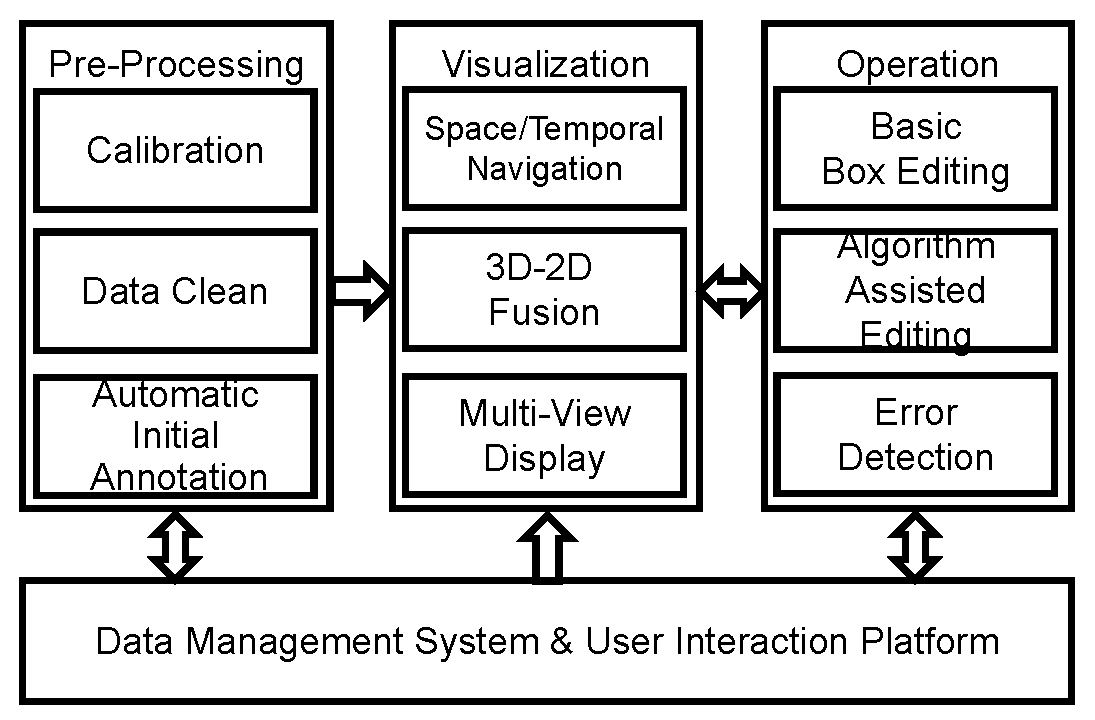
\includegraphics[width=0.45\textwidth]{./platform}\\ %\vspace{-0.3cm}
	\caption{Annotation platform}
	\label{fig:main-arch}
	\vspace{-0.3cm}
\end{figure}


2D/3D box-based units for editing 

Visualization methods are developed to improve VR

automation tools are developed for scalability and extension 

room for improvement: 

This paper presents 
\begin{enumerate}
	
	\item.
	\item.
	\item.
	
\end{enumerate}

The contributions of this work include
\begin{enumerate}

	\item developing an open-source 3D point annotation platform featuring  well-designed visualization and convenient operations.
	\item developing a series of functions such as auto-shrink, boundary-aware rotation and smart box initialization etc. to enable fast and accurate 3D box annotating.
	\item developing a novel registration-based inter-frame annotation transfer method.
\end{enumerate}

The rest of this paper is organized as follows. Section






\begin{comment}



%3D environment understanding plays an important role in the autonomous driving. There are many ways to build the 3D environment, which can be divided into 2 categories, including sensor-based and algorithm-based.
Recently, 3D environment understanding is gaining the attention in the research areas and industrial applications, like autonomous driving, etc. The 3D environment is often represented as point clouds. And the density of the point clouds reflects the quality of the 3D environment. A common method of obtaining 3D point clouds is by laser scanners, like LiDAR, etc. The labeling process of the point clouds have to deal with the following limitations/challenges:
\begin{figure}[htbp]
 \centering
 % Requires \usepackage{graphicx}
 %\resizebox{\linewidth}{!}{
 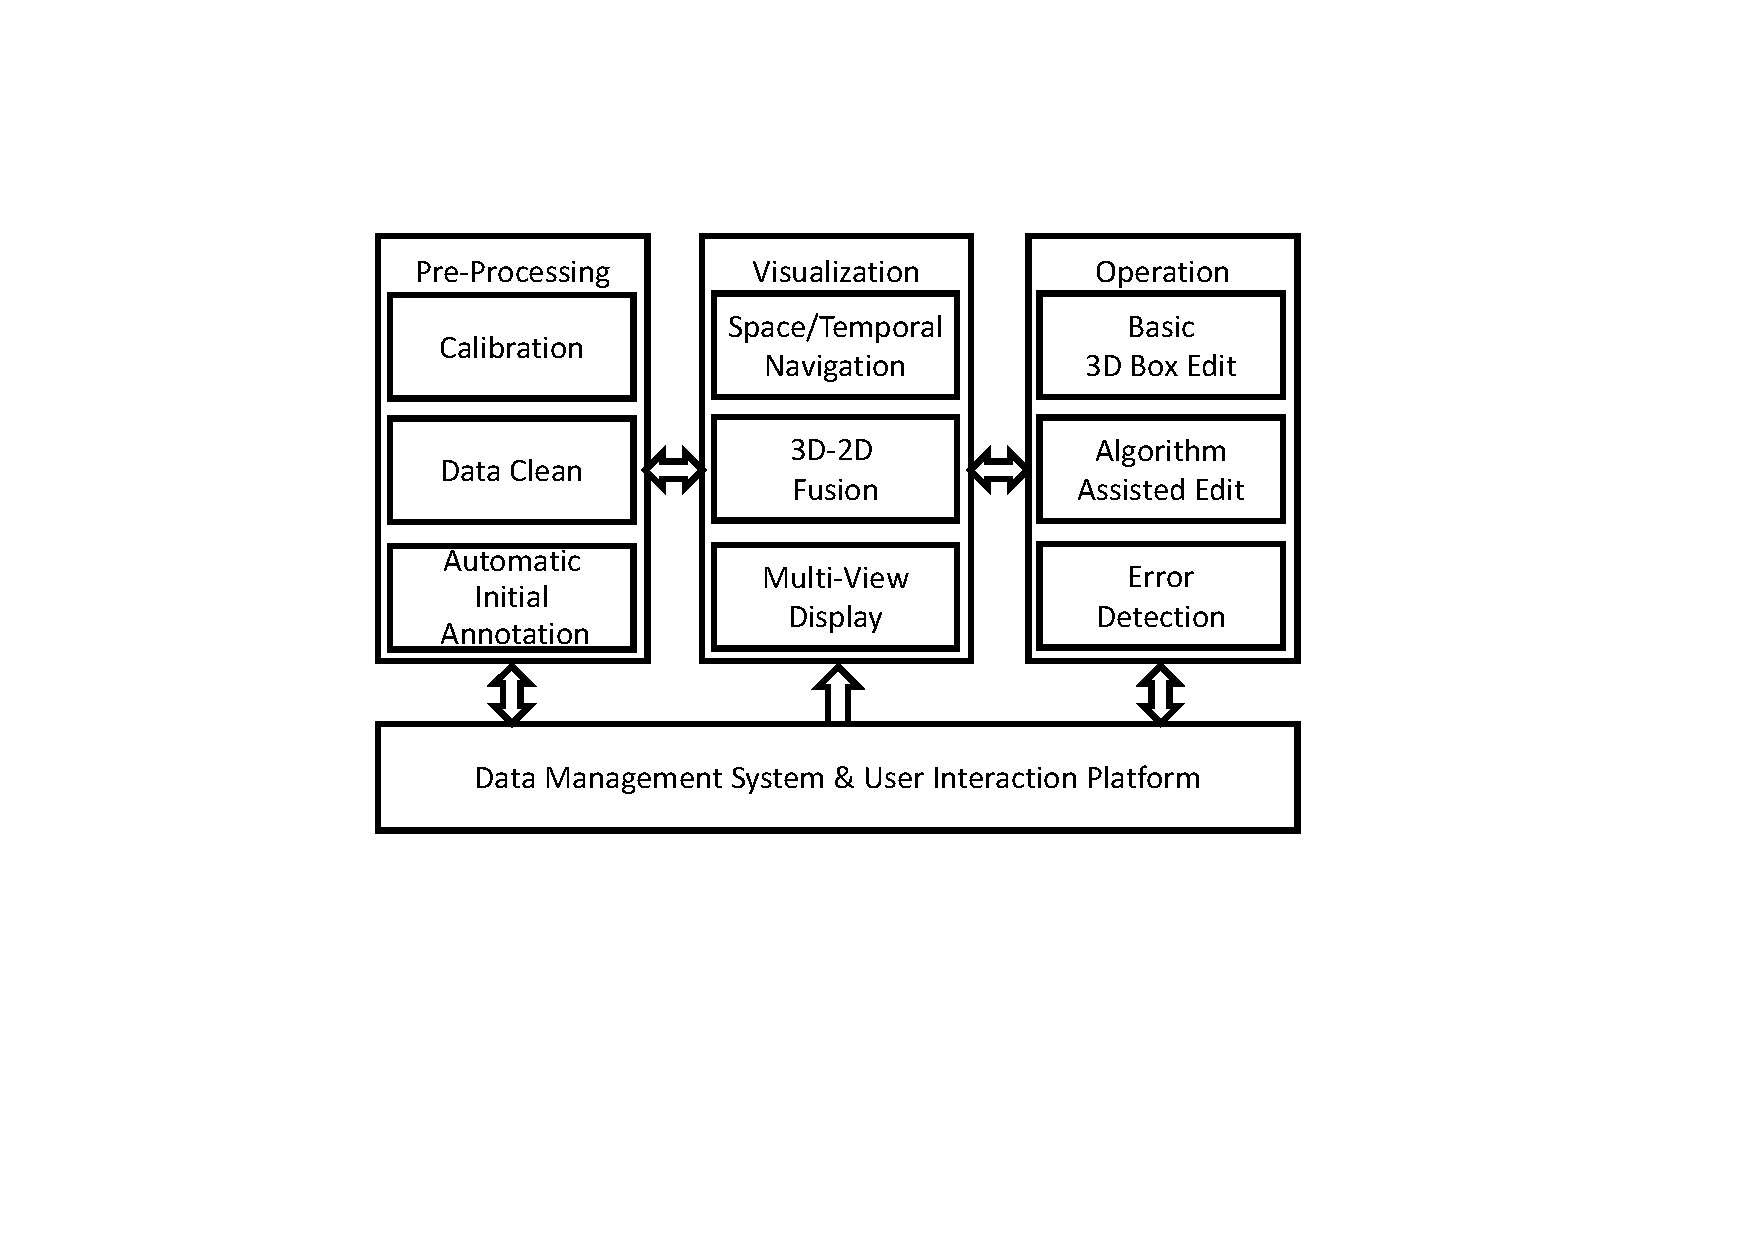
\includegraphics[width=0.45\textwidth]{./figures/arch}\\ %\vspace{-0.3cm}
 \caption{An illustration of our annotation platform. Our annotation procedure includes 3 modules, which are pre-processing, visualization and operation, respectively. The pre-processing module is used to obtain the sensor calibration information, filter the noises in data, and initialize AI method-based annotation results. The visualization module is utilized to assist data annotation. And the operation module implements the 3D bounding box annotation in the point clouds with algorithm assistance and also checks the annotation error.}
 \label{fig:arch}
 \vspace{-0.3cm}
\end{figure}

\begin{enumerate}
  \item Irregular density point cloud. In practical, the density of point clouds depends on distance between the sensor and measured objects, sensor type, and reflectivity of the measured objects, etc. Therefore, how to solve the different density of point clouds, including sparse and dense, becomes crucial.
  \item High-precision annotation. Compared with 2D image annotation, the annotation information of 3D point clouds becomes more complexity. It includes scale at each dimensionality axis, and heading angle of the object. How to obtain the accurate annotation information becomes important.
  \item Rich categories of object. The data-driven-based methods can distill the knowledge from the rich categories of the dataset, so that these methods can keep the favorable performance. The number of these objects is numerous. How to quickly annotate and balance these objects is also a critical issue.
  \item Reasonable data structure. The reasonable annotation data structure can efficiently decrease the store space and boost the speed of access.
  \item Flexible tool. Labeling the 3D objects is an enormous work, which includes annotation large amounts of objects and operation instructions for users. Therefore, developing a flexible labeling tool is much more important.
\end{enumerate}

The resolution of 3D point clouds is a formidable limitation for 3D annotation. Each frame point clouds obtained by LiDAR, like Velodyne, RoboSense, etc., has at least 10K 3D points. The measurement radius of  LiDAR is larger than 150 meters. So there are quite a few objects with a small number of points, extremely fewer than 10 points. These low-resolution 3D objects are even beyond the perception ability of humans. Another limitation is how to improve the annotation efficiency of the same object in consecutive frames, especially when the objects being farthest away from the sensor are with low-resolution 3D points.

An flexible annotation tool can improve the annotation efficiency and dataset quality. A considerable amount of research has been done on how to annotate 3D point clouds, like PointAtMe~\cite{pointatme}, LabelMe3D~\cite{LabelMe3D}, etc., during the last decade. The flexible annotation tool should be with easily applicable, intelligible and favorable visibility, as shown in the Fig.~\ref{fig:arch}. The intelligible plug-in of the annotation toolkit can promote the speed of the annotation process. The favorable visibility can raise the quality of the dataset, specifically in balancing the number of objects.

In this paper, we propose an efficient 3D point clouds annotation tool, with flexible operation, semi-autonomous annotation, and rapid deployment, to improve the annotation efficiency and assure the dataset quality. The contribution of this work as shown in the following.
\begin{itemize}
  \item Developing a flexible operation annotation tool for 3D point clouds;
  \item Developing a semi-autonomous method to annotate the same objects in the consecutive frames;
  \item Developing an intelligent plug-in being used to count the number and type of labeled objects.
\end{itemize}

The rest of this paper is organized as follows. Section~\ref{Realtedwork} introduces the related work on 3D objects annotation methods.
Section~\ref{setup-statement} describes the system setup and problem statement. Section~\ref{Approach} presents the proposed method.
Section~\ref{result} provides the experiment results and discussions. Section~\ref{conclusions} concludes this paper and outlines future work. To facilitate future research, the code has been released at "\url{http://www.baidu.com}".

\end{comment}



\begin{table*}[ht]
	\caption{A brief summary on 3D point clouds annotation tools}
	\resizebox{1.0\textwidth}{!}{
	\begin{tabular}{c||p{1cm}<{\centering}|p{1cm}<{\centering}|p{1cm}<{\centering}|p{1cm}<{\centering}|p{1cm}<{\centering}|p{1cm}<{\centering}|p{1cm}<{\centering}|p{1cm}<{\centering}
			||p{1cm}<{\centering}|p{1cm}<{\centering}|p{1cm}<{\centering}|p{1cm}<{\centering}|p{1cm}<{\centering}}
		\hline \hline
		\multirow{2}{*}{} & \multicolumn{8}{c||}{Visualization}                         & \multicolumn{5}{c}{Operation}                 \\
		\cline{2-14}                       &3D Space/ Time Navigation & Main View Focus Mode   & Box \& Object Coloring & Top/Side/ Front Views  &Photo Context with 3D-2D Fusion  &Focused Context & Multi Camera w/~Auto Switching & Stream Play with Object Locking    & Box Degrees of Freedom & Auto box Initialization& Sub-view editing & Semi Auto Fitting  & Annotation Transfer \\  \hline
		PointAtMe~\cite{pointatme}         &                 $\surd$  & $\times$               &  $\times$              &  -                     & $\surd$*                        &  $\times$      &  $\times$                       &  $\times$                       & 9                      &     -                    &   n/a            &   -                 &   -            \\ \hline
		3D BAT~\cite{Zimmer20193DBA}       &                 $\surd$  & $\times$               &  $\surd *$             &  $\surd$*              & $\surd$                         &  $\times$      &  $\surd$*                       &  $\times$                       & 9                      &     -                    &   -              &   -                 &   ++            \\ \hline
		LATTE~\cite{Wang2019LATTEAL}       &                 $\surd$  & $\times$               &  $\times$              &  $\times$              & $\surd$*                        &  $\times$      &  $\times$                       &  $\times$                       & 5                      &     ++                   &   -              &   -                 &   ++            \\ \hline
		Supervise.ly~\cite{SUPERVISELY}    &                 $\surd$  & $\times$               &  $\surd *$             &  $\surd$               & $\surd$                         &  $\times$      &  $\times$*                      &  $\times$                       & 9                      &     -                    &   ++             &   -                 &   unknwon       \\ \hline
		scale.ai~\cite{scale}              &                 $\surd$  & $\times$               &  $\surd *$             &  $\surd$               & $\surd$                         &  $\times$      &  $\surd$*                       &  $\times$                       & 7                      &     unknown              &   unknown        &   -                 &   unknown       \\ \hline
		Playment.io~\cite{Playment}        &                 $\surd$  & $\times$               &  $\surd *$             &  $\surd$               & $\surd$                         &  $\times$      &  -                              &  $\surd$                        & -                      &     -                    &   ++             &   -                 &   ++            \\ \hline
		\textbf{SUSTech Points}            &                 $\surd$  & $\surd$                &  $\surd$               &  $\surd$               & $\surd$                         &  $\surd$       &  $\surd$                        &  $\surd$                        & 9                      &     +++                  &  +++             &  +++                &  +++            \\ \hline \hline
	\end{tabular}
	}
	\begin{tabular}{p{17.5cm}}
		The symbol ``$\surd$'' means the tool has the feature, ``$\times$'' otherwise, ``$\surd$*'' indicates partial support. The number of ``$\textbf{+}$''s represent the performance of the feature, the more the better, ``-'' means lacking of the feature. We briefly introduces features below:
		
		\begin{enumerate}
			\item ``Main View Focus Mode": a selected object can be zoomed in and centered in main view with one click.
			
			\item ``Stream play'': the data can be played as a video
			\item ``Object Locking": an object can be selected automatically in all frames at stream  playing. 
			
			\item ``Focused context'': The part of photo context focusing on current object under editing is displayed in a single sub-view
			
			\item ``Camera Auto-Switching'': photo context can be automatically switched among multiple cameras when navigating objects. 
			
			\item ``Auto box initialization": box can be fitted automatically to the object at creating.
			
			\item ``Sub-view editing": editing box on projective sub-views.
			
			\item ``Semi Auto Fitting": the box can be fitted  automatically  to object when editing (\textit{e}.\textit{g}. rotating and resizing).
			
			\item ``Annotation Transfer": to transfer annotation across frames by an automatic or semi-automatic way.
			
		\end{enumerate}

		All other feature shall be clear by the name itself.
		
		% after \\: \hline or \cline{col1-col2} \cline{col3-col4} ...
	\end{tabular}
	\label{tab:annotationMethods}
	\vspace{-0.5cm}
\end{table*}


\section{Related work}
\label{Realtedwork}
According to the types of annotation equipment, much of the research in the 3D annotation area in recent years can be classified as 2D-screen based and VR (virtual-reality) based methods. The table~\ref{tab:annotationMethods} gives the details comparison on current popular 3D point clouds annotation methods. In this table, the first 6 methods and ours are open source, and the remainning methods are commercial.
\subsection{2D-screen based annotation method}
2D-screen based methods can guarantee the 3D annotation quality and are without additional equipment to finish specific annotation tasks.
Details on these methods include the 2D-3D fusion-based and pure 3D-based annotation.
2D-3D fusion-based methods need the accurate spatial transformation relationship between 2D cameras and 3D sensors.
The spatial transformation relationship is calibrated by the stereo-vision algorithms, including Zhang's method~\cite{zhangzhegnyou}, Camera-LiDAR calibration~\cite{roadCalibration}, \emph{etc.}
But the performance of annotation strongly depends on the 2D-3D correspondence estimated from each sensor data. In addition, the 3D point are discrete and cannot find the accurate corresponding pixels at the image, which can increase the error of calibration and projection. A slice of these methods can only process the specific scenarios, like static scenarios, indoor scenarios, and so on.

Another kind of methods directly operates at the layer of 3D point clouds.
The method proposed by Yu \textit{et al.}~\cite{yu2012efficient} selects some points around the 2D projection of the object in 3D environment, which can approximately annotate the 3D object according to the structure-aware information. The cluster-based methods and segmentation-based method stand for the semi-autonomous and fully autonomous annotation method.
These methods outperform the VR-based annotation methods. However, these methods are with higher time consuming and computation complexity~\cite{pointatme}. It is worth noting that the method~\cite{monica2017multi} is the only one seriously evaluating the speed of their annotation tool. And we also adopt the metric~\cite{monica2017multi} to evaluate the speed of our label tool.
\subsection{VR-based annotation method}
VR equipment is helpful for the 3D environment understanding. However, the VR-based 3D annotation mathods are with the following limitations, including big annotation errors, highly time consuming. The VR can afford the immersion experience during wearing VR equipment. Taking advantages of VR, VR-based methods for 3D annotation are proposed in quite a few works~\cite{pointatme,wilkes20123dVR,coffey2011interactiveVR}. Since the VR-based methods depend on the hand gestures and 2 controllers to tune the bounding box of the 3D objects, it is difficult to accurately locate the boundaries of objects and implement fine-tuning the attitude, size, and angle in the short time. During the trade-off between efficiency and quality, the labeled bounding box by the VR-based methods is with bigger errors than that of the VR-free methods.

Another reason of the limitations is the point clouds belonging to the same object within an appropriate bounding box.
It needs multiple repeat operations to select the proper boundary points.
Specifically, the labeling process of the complex objects with irregular boundaries, like trees, zebra lines, etc., becomes more difficult than that of other objects with regular boundaries, such as cars, vans, and so on.

These 2 limitations increase the time consuming and decrease the annotation quality of 3D objects.
\subsection{The framework of annotation method}
The framework of annotation method includes explorer-based and software-based. The explorer-based framework is flexible to users for labeling 3D objects, which is based on the elements of the Web page. Therefore, the annotation framework, like LabelMe3D~\cite{LabelMe3D}, our proposed method, \emph{etc.}, can adaptively perform at any computer without additional operations. The software-based methods, like AppoloSuite~\cite{SUPERVISELY,wang2019apolloscape}, also need additional component that can ensure to execute. And it is difficult to synchronously and instantly update, which maybe cause the inconsistency of data, or other unpredictable results.

In this work, our proposed method directly annotate the objects at the 3D point clouds layer with the explorer-based framework. Our proposed method is with a convenience visualization module and intelligent operation module, as shown in table~\ref{tab:annotationMethods}, which can successfully process the trade-off between time-consuming and data-quality.

\section{System Architecture and Features}

\subsection{System Architecture}
Our platform focus on 3D bounding box and tracking ID annotation. For bounding box our platform supports 9 degrees of freedom editing. 

We use web-based architecture. A annotator works with a web browser. The raw data shall be put on server beforehand. 

The web server is implemented in Python and relies on CherryPy\cite{cherrypy} web framework. The frontend relies on \texttt{WebGL} library Three.js\cite{threejs}. The backend mainly serves data managements functions, the frontend implements almost all features described in this section.
\begin{comment} Fig.~\ref{fig:arch_layer} depicts the overview of the architecture.

\label{3D annotation tool}
\begin{figure}[htp]
	\centering
	  \vspace{-0.1cm}
	% Requires \usepackage{graphicx}
	%\resizebox{\linewidth}{!}{
	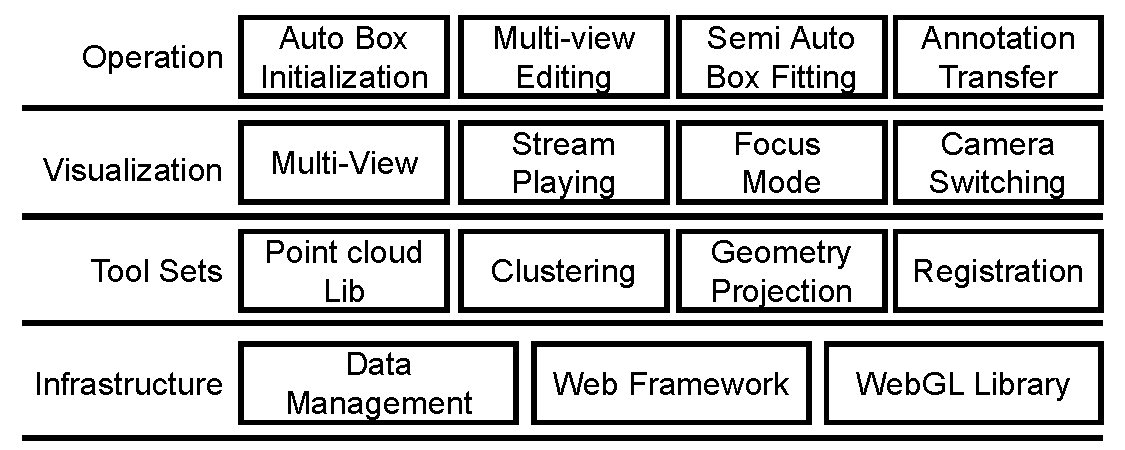
\includegraphics[width=1.0\linewidth]{./arch_layer}\\ %\vspace{-0.3cm}
	 \caption{Layered architecture of our annotation platform.}
		\label{fig:arch_layer}
		\vspace{-0.3cm}
   \end{figure}
\end{comment}

\subsection{Visualization}

Visualization is important for both 3D box editing and reviewing. Fig.~\ref{fig:main-ui} shows the main user interface of our platform. We describe details of visualization features in following subsections.

\begin{figure}[!t]
	\centering	
	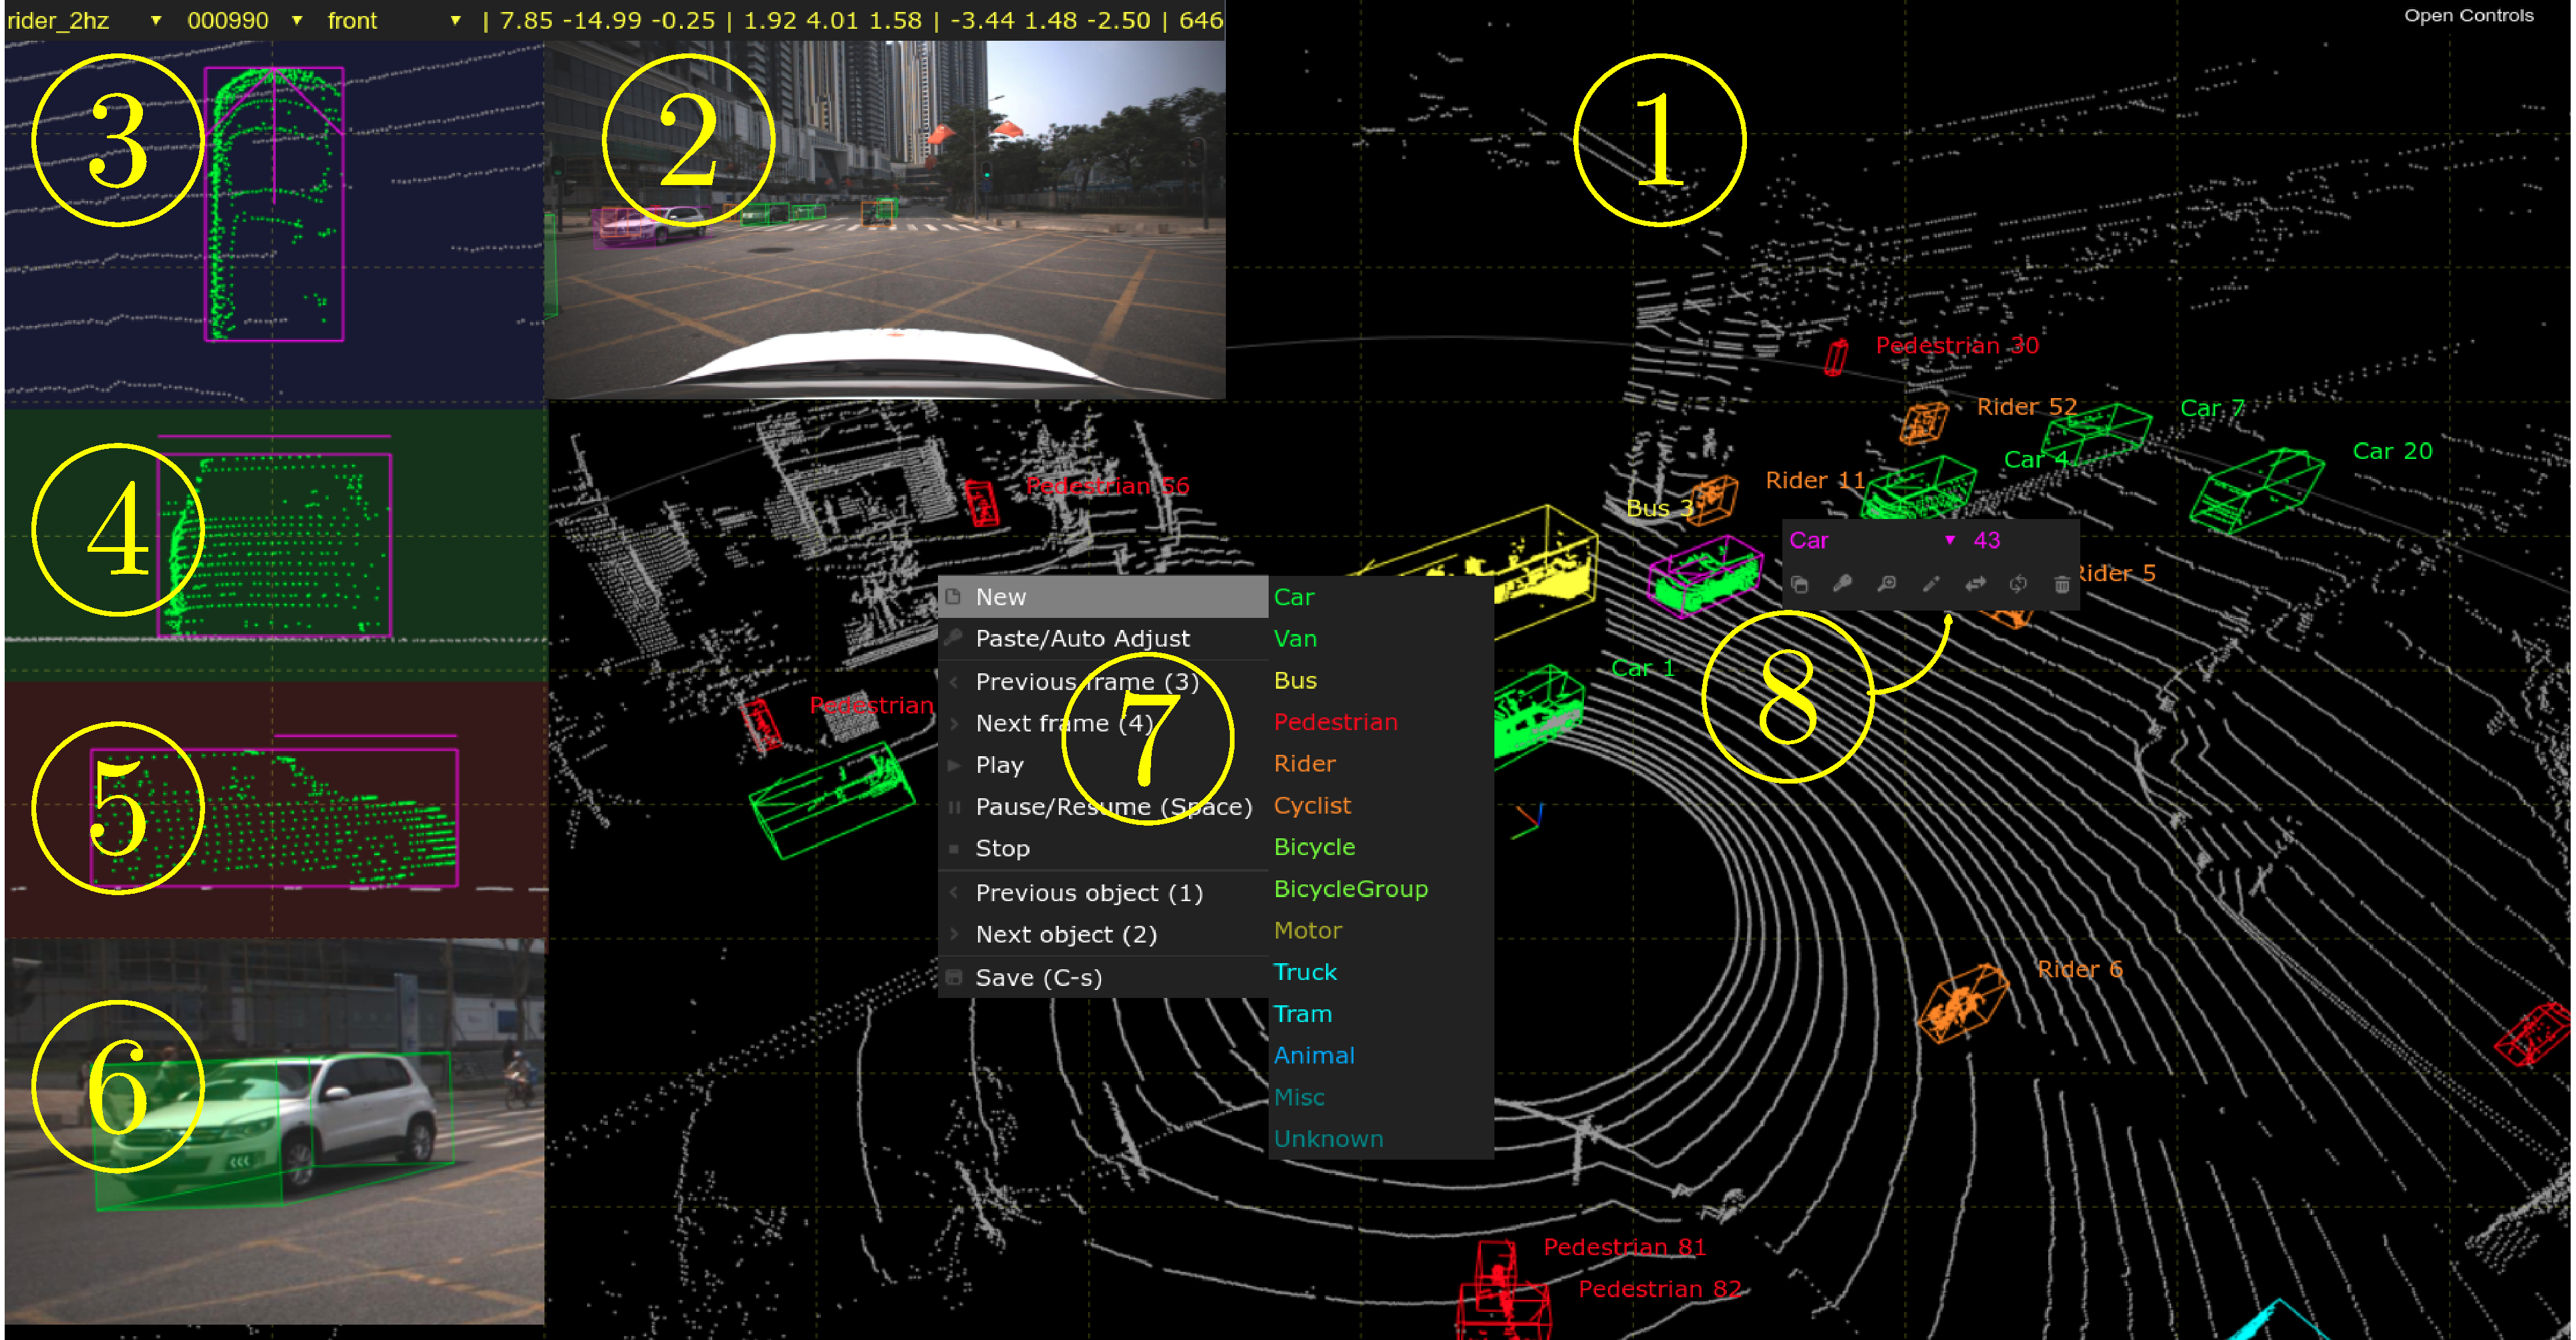
\includegraphics[width=\linewidth]{./figures/main-ui}\\
	\caption{Main UI, \textcircled{1} is perspective view, \textcircled{2} is photo context, which is resizable and can automatically switch among multiple camera images, \textcircled{3} is top view, \textcircled{4} is front view, \textcircled{5} is side view, \textcircled{6} is focused photo context which follows selected object automatically. \textcircled{7} is context menu, \textcircled{8} is floating fast toolbox.}
	\label{fig:main-ui}
\end{figure}

\subsubsection{Sub-views}
\label{section:sub-views}
We split the main window into 1 main view and 5 sub-views, as shown in Fig.~\ref{fig:main-ui}. The top,front and side projective views are displayed on left side with background hidden. Beside context photo view on the top, an extra focused context sub-view is also provided(bottom left sub-view). Annotated 3D boxes are projected to these 2 photo context sub-views.




\subsubsection{Focus-mode}
We provide a focus mode to help check object details. When activated through fast toolbox(\textcircled{8} in Fig.~\ref{fig:main-ui}),the target object is automatically centered and zoomed in, most background hidden, while all editing features still applicable. Without this feature a user has to pan,  zoom and rotate the main view often, which we think is laborious.

\subsubsection{Camera auto-switching}
It's common to have multiple cameras in nowadays autonomous driving car setup, \cite{Zimmer20193DBA} displays all camera images on top of the main view, some displays only one \cite{scale}. we choose the latter way but with an automatic camera switching feature. Specifically when an object is selected in point cloud, the most relevant camera image is displayed. Manual camera selection is also possible. Note that this feature needs the calibration data to be available.

\subsubsection{Object Coloring}
All boxes and object points can be colored by categories. Selected object (object under editing) are highlighted with a different color.

\subsubsection{Navigation}
\label{section:navigation}
A user can navigate in 3D space, or in time  by navigating previous or next frame. 

\subsubsection{Stream Play}
\label{section:streamplay}
A user can play the data (by scenes) like a video.

\subsubsection{Object locking}
\label{section:object-locking}
When playing, selected object are locked (\textit{i}.\textit{e}. selected in all frames).

\subsubsection{Box information}
Box details (scene, frame, object category, coordinates, dimension, direction and points number) are shown on top of the main window.
 
\subsection{Basic 3D Box Editing}

\subsubsection{Creating a box}
\label{section:create-box}
A user can create a new box by right clicking on the object  and then select object type on popup context menu. Our platform provide the following features to help create box easily:

\begin{enumerate}
	\item The initial box direction (yaw) is upright along the main view. It's common that a group of vehicles have similar or reverse directions in one scene, so adjust the view angle of the main view properly can save a lot time.
	\item A box prototype (in accordance with the object type) is placed on mouse position.
	\item A Euclidean distance based growing algorithm is invoked to include all points of the object.
	\item An auto-fitting algorithm (\ref{section:auto-fitting}) is used to shrink the box in case there is margin between the box and the object.
\end{enumerate}

Note that \emph{for most cases, the annotation is almost done with this single operation}.

Different from "one-click-annotation" of LATTE~\cite{pointatme}, which uses clustering algorithm to find points of the object under clicking, our method uses prototype to overcome difficulties when the points is too sparse for a clustering algorithm to work.

A user can also create a new box by drawing a rectangle on main view,  enclosing relevant points. The box is created by setting direction  as described above and fitted to enclosed points. The object type is automatically set by simply matching the object dimension to prototypes.


\subsubsection{Edit in perspective view}

When an object is selected, a floating \emph{fast toolbox} shows next to it, as shown in Fig.~\ref{fig:main-ui}. A user can change object type, tracking id, activate focus mode, among others.

For tracking ID, A user  can input or select existing value in fast toolbox, or select 'auto' option  letting the platform to generate a new ID unique in the scene.


A user can click a selected object or the button on fast toolbox to enable box editing, drag the handlers as show in Fig.~\ref{fig:box-mouse-edit} to resize,rotate or move the box. Corresponding keyboard shortcuts are also provided.
 

\begin{figure}[t]
	\centering
 \resizebox{\linewidth}{!}{
	\begin{subfigure}{0.3\linewidth}
		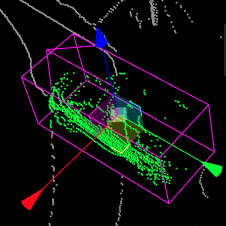
\includegraphics[height=2.5cm]{./figures/box-move}\\
		\caption{move}
	\end{subfigure}
	\begin{subfigure}{0.3\linewidth}
		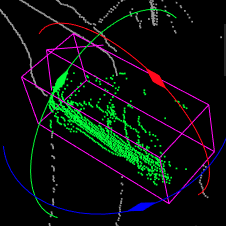
\includegraphics[height=2.5cm]{./figures/box-rotate}\\
		\caption{rotate}
	\end{subfigure}	
	\begin{subfigure}{0.3\linewidth}
		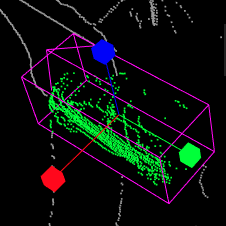
\includegraphics[height=2.5cm]{./figures/box-resize}\\
		\caption{resize}
	\end{subfigure}
}
	\caption{Box editing in perspective view}
	\label{fig:box-mouse-edit}
\end{figure}


\begin{figure}[t]
	\centering
	\resizebox{\linewidth}{!}{
		\begin{subfigure}{0.3\linewidth}
			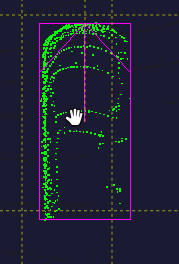
\includegraphics[height=4.cm]{./figures/subview-move-xy}\\
			\caption{move}
		\end{subfigure}
		~
		\begin{subfigure}{0.3\linewidth}
			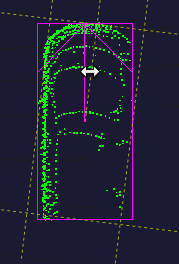
\includegraphics[height=4.cm]{./figures/subview-rotate-xy}\\
			\caption{rotate}
		\end{subfigure}
	    ~
	    \begin{subfigure}{0.3\linewidth}
	    	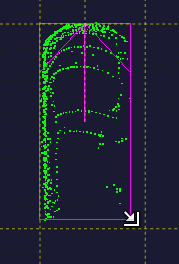
\includegraphics[height=4.cm]{./figures/subview-resize-xy}\\
	    	\caption{resize}
	    \end{subfigure}	
	}
	\caption{Box editing in projective sub-view}
	\label{fig:box-mouse-edit-subview}
\end{figure}

\subsubsection{Edit in projective sub-views}
Editing in perspective view is inconvenient,  a user has to change viewpoint often for better operation. As shown in Fig.~\ref{fig:main-ui} the annotation is clearly shown in the sub-views, thus we enable editing directly on these sub-views to make a better editing experience. A user can rotate, resize or move the box by mouse operation, as shown in Fig.~\ref{fig:box-mouse-edit-subview}.
All operations can also be done with keyboard shortcuts.



\subsection{Assistant algorithms}


\subsubsection{Semi-auto box fitting}
\label{section:auto-fitting}
When a box is being resized or rotated, our platform can fit the box to the object automatically. This is done by finding the minimal box enclosing all points. For those objects with few points, the box need to be larger than fitted, it can be adjusted manually. Fig.~\ref{fig:boundary-aware-rotation} shows box fitting at rotating, note all points of the object are kept inside after rotated. With this feature, \emph{to annotate a new object is as easy as to enclose all pionts first and rotate once (\ref{section:create-box})} in most cases.

Note that a direct manner to find the minimal box may fail when ground plane is present. As an example, in Fig.~\ref{fig:box-before-rotate}, if the ground plane is counted in, a new fitted box after rotation will be too large. One solution is to remove ground plane with algorithms, but it's not reliable when the ground is not smooth (as can be seen often in KITTI data set\cite{Geiger2012CVPR} where many cars parked on roadside).

We use a simple yet effective method to solve this problem. Specifically, we  ignore the most bottom part (0.2m by default) of the object when calculating the box dimension (x-y plane). Since a user is annotating the object, the pose of the object must be already roughly correct, so the  ground points can be removed effectively with this method. In traffic scenarios almost all objects are much higher than 0.2m, so the estimation of dimension is  seldom affected. For object height (z axis) we compensate the 0.2m part after the calculation. 


\begin{figure}[t]
	\centering
	
	\begin{subfigure}[t]{0.2\linewidth}
		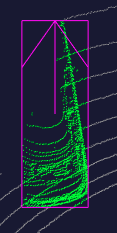
\includegraphics[height=4cm]{./figures/points-enclosed}
		\caption{}
		\label{fig:box-before-rotate}
	\end{subfigure}\hfill
	\begin{subfigure}[t]{0.2\linewidth}
		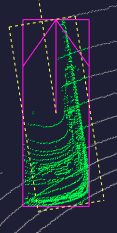
\includegraphics[height=4cm]{./figures/adjust-naively}
		\caption{}
		\label{fig:box-rotate-in-subview}
	\end{subfigure}\hfill
	\begin{subfigure}[t]{0.2\linewidth}
		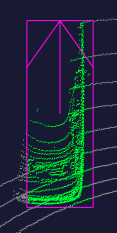
\includegraphics[height=4cm]{./figures/rotate-fail}
		\caption{}
		\label{fig:box-rotate-naively}
	\end{subfigure}\hfill
	\begin{subfigure}[t]{0.2\linewidth}
		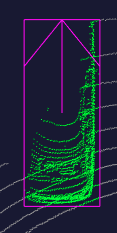
\includegraphics[height=4cm]{./figures/rotate-success}
		\caption{}
		\label{fig:box-rotate-correctly}
	\end{subfigure}\hfill
	\caption{Box auto-fitting on rotation. For box in \ref{fig:box-before-rotate}, which encloses all points of a car, if it's rotated counter-clockwise naively(\ref{fig:box-rotate-in-subview}), part of the object will go outside(left lower part of \ref{fig:box-rotate-naively}), our platform can automatically fit the box as shown in (\ref{fig:box-rotate-correctly})}
	\label{fig:boundary-aware-rotation}
	\vspace{-0.3cm}
\end{figure}


\subsubsection{Annotation transfer among related frames}
\label{semi-auto-anno}
In autonomous driving scenario, data sets are often organized by scenes\cite{Caesar2019nuScenesAM,Patil2019TheHD,lyft2019}. A scene is a sequence of frames shot at one continuous period of time. There are much similarities between neighboring frames, which makes it possible to transfer annotations among them. \cite{Zimmer20193DBA} copies annotations to next frame directly and let user do the adjustment.\cite{Wang2019LATTEAL} uses box estimation algorithm to automatically adjust the box, reusing previous annotated object size if appropriate. Our platform takes this way further by invoking registration algorithm \cite{Yang2016GoICPAG} to automatically adjust the position and rotation, reusing both the size and rotation previously annotated. In most cases our method produces  accurate enough annotation result.

A user needs to first select (copy) a reference box, then paste it at appropriate position in target frame. A registration algorithm is invoked to compute the relative transform relation between the reference and target object, then the box in the target frame is adjusted accordingly.

The reference and target objects are cropped out at a 1.2 scale ratio and all points are transformed to their corresponding box coordinates system before input to registration algorithm. Fig.~\ref{fig:annotation-transfer} shows an transfer example.

The performance of this function depends on the registration algorithm.  Empirically it works well when the reference object and the target object have similar view angles. Several adjustments may be requered if the initial position is deviated too much.

\begin{figure}[t]
	\centering
	\begin{subfigure}[t]{0.18\linewidth}
		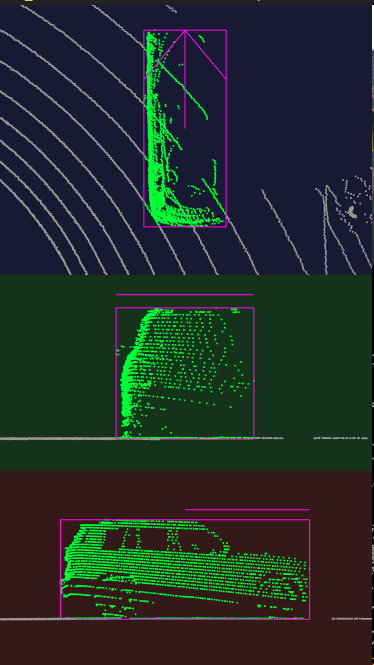
\includegraphics[height=4cm]{./figures/reg-ref-3d}\\
		\caption{}\label{fig:box-ref}
	\end{subfigure}\hfill
	~
	\begin{subfigure}[t]{0.18\linewidth}
		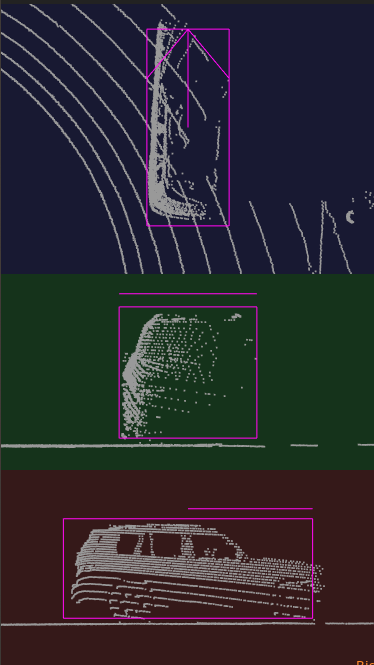
\includegraphics[height=4cm]{./figures/reg-input-3d}\\
		\caption{}\label{fig:box-source}
	\end{subfigure}\hfill
	~
	\begin{subfigure}[t]{0.18\linewidth}
		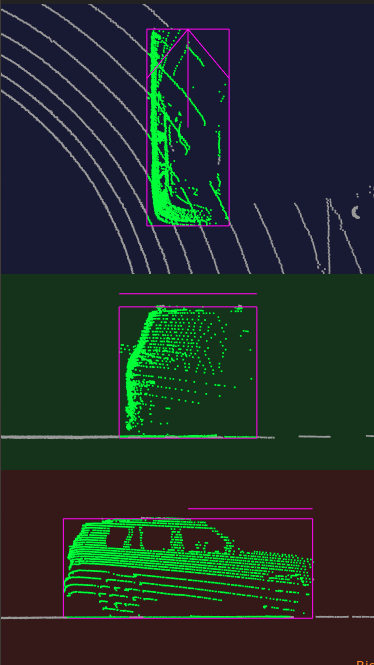
\includegraphics[height=4cm]{./figures/reg-result-3d}\\
		\caption{}\label{fig:box-output}
	\end{subfigure}\hfill
	~
	\begin{subfigure}[t]{0.18\linewidth}
		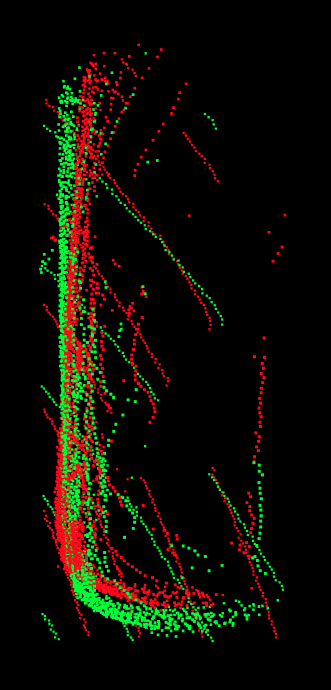
\includegraphics[height=4cm]{./figures/reg-input}\\
		\caption{}\label{fig:reg-input}
	\end{subfigure}\hfill
	\begin{comment}
	~
	\begin{subfigure}[t]{0.18\linewidth}
		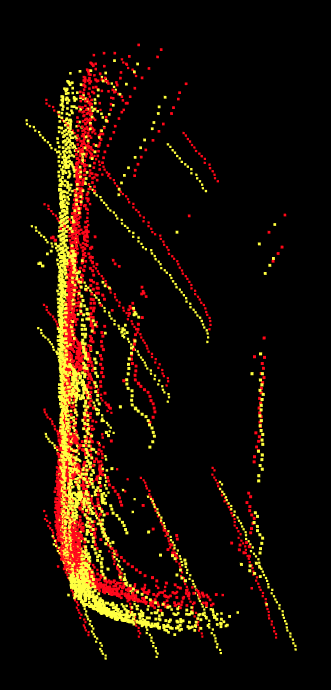
\includegraphics[height=3cm]{./figures/reg-tran}\\
		\caption{}\label{fig:reg-tran}
	\end{subfigure}\hfill
	~
	\begin{subfigure}[t]{0.18\linewidth}
		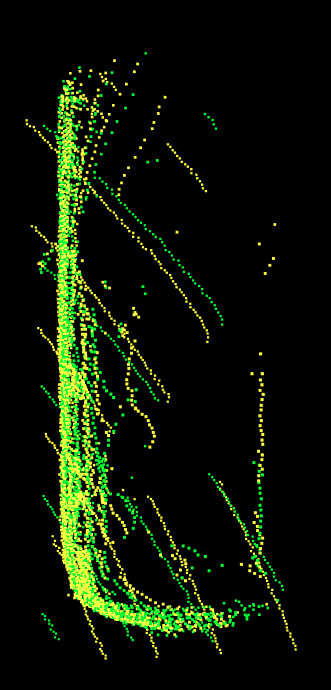
\includegraphics[height=3cm]{./figures/reg-result}\\
		\caption{}\label{fig:reg-output}
	\end{subfigure}\hfill
	\end{comment}
	
	\caption{Registration based bounding box transfer. \ref{fig:box-ref} is the reference object and its bounding box, \ref{fig:box-source} is the object in another frame with a initial  bounding box, \ref{fig:box-output} is the result of box being adjusted by annotation transfer,\ref{fig:reg-input} is the corresponding registration input after coordinates transformed.}
	\label {fig:annotation-transfer}
\end{figure}


We describe the box transformation procedure in the remaining part of this section. 
Given source and target objects (denoted by $\mathcal{S,T}$ respectively)and their bounding boxes ($b_s,b_t$), a registration algorithm finds the transform matrix $T$ to match $\mathcal{S}$ with $\mathcal{T}$ , minimizing a distance function $dist$,
$$dist(T(\mathcal{S}),\mathcal{T})$$
where we represent points of $\mathcal{S,T}$ in their corresponding bounding box coordinates $B_s$ and $B_t$, the world coordinate system is denoted as $B_w$. Note that the box itself is identical to box coordinates system (\textit{i}.\textit{e}. $b_s$ is identical to $B_s$) since we concern only the rotation (correspond to 3 axes) and position (correspond to the origin point) of the box.

Assume point $s \in \mathcal{S}$ corresponds to $t \in \mathcal{T}$ after registration, then


\begin{align}
T s^{B_s} &= t^{B_t}\\
T B_s^{-1}s^{B_w} &= t^{B_t} \label{eq:eq1}
\end{align}

where $s^{B_s}$ means s represented in $B_s$ coordinate system.

If we denote the new coordinate system of $\mathcal{S}$ as $B'_s$, then
\begin{align} 
s^{B'_s} &= t^{B_t}\\
(B'_s)^{-1}s^{B_w} &= t^{B_t} \label{eq:eq2}
\end{align}


by Eq.~\eqref{eq:eq1} and Eq.~\eqref{eq:eq2}, we have

\begin{align}
{B'_s} & = (T B_s^{-1})^{-1}\\
       & = B_s T^{-1} \label{eq:eq5}
\end{align}

If we use the reference object as target, object under annotation as source, Eq.~\eqref{eq:eq5} tells us we should apply the reverse transform of registration to the coordinates system, that is, to the box.


%\subsection{Proposed annotation procedure}

\section{Results and Evaluation}
\label {Metrics}

The evaluation consists of 3 parts:
\begin{enumerate}
	\item Evaluation of review efficiency, we show that errors or inaccuracies are easy to identify through the visualization functionalities.
	\item Evaluation of annotation efficiency, we show that annotation time and accuracy is better compared to other available tools.
	\item Evaluatoin of transfer annotation, we show that transfer annotation generate accurate enough results.
\end{enumerate}

\subsection{Review Efficiency}
We use examples from KITTI 3D Object Detection data set \cite{Geiger2012CVPR}  to demonstrate the effectiveness of checking annotation accuracy with our platform. We choose the same scene as show in  Fig. 5 of \cite{pointatme}.

Note although our platform supports all 9 degrees of freedom for 3D box, only 7 are labeled in KITTI data set, with pitch and tilt ignored, so in our evaluation we also ignore these 2 angles for fairness.

As show in Fig.~\ref{fig:annocheck}, we demonstrate that thanks to the 4 sub-views (Section~\ref{section:sub-views}) errors or inaccuracy spots are immediately and clearly identified by just navigating the objects one by one (Section~\ref{section:navigation}).

Tracking IDs can also be easily checked with the help of object locking (\ref{section:object-locking})  and stream-play(\ref{section:streamplay}) feature. For brevity we choose not to show examples here.

\begin{figure}
	\centering
	\begin{subfigure}{0.3\linewidth}
		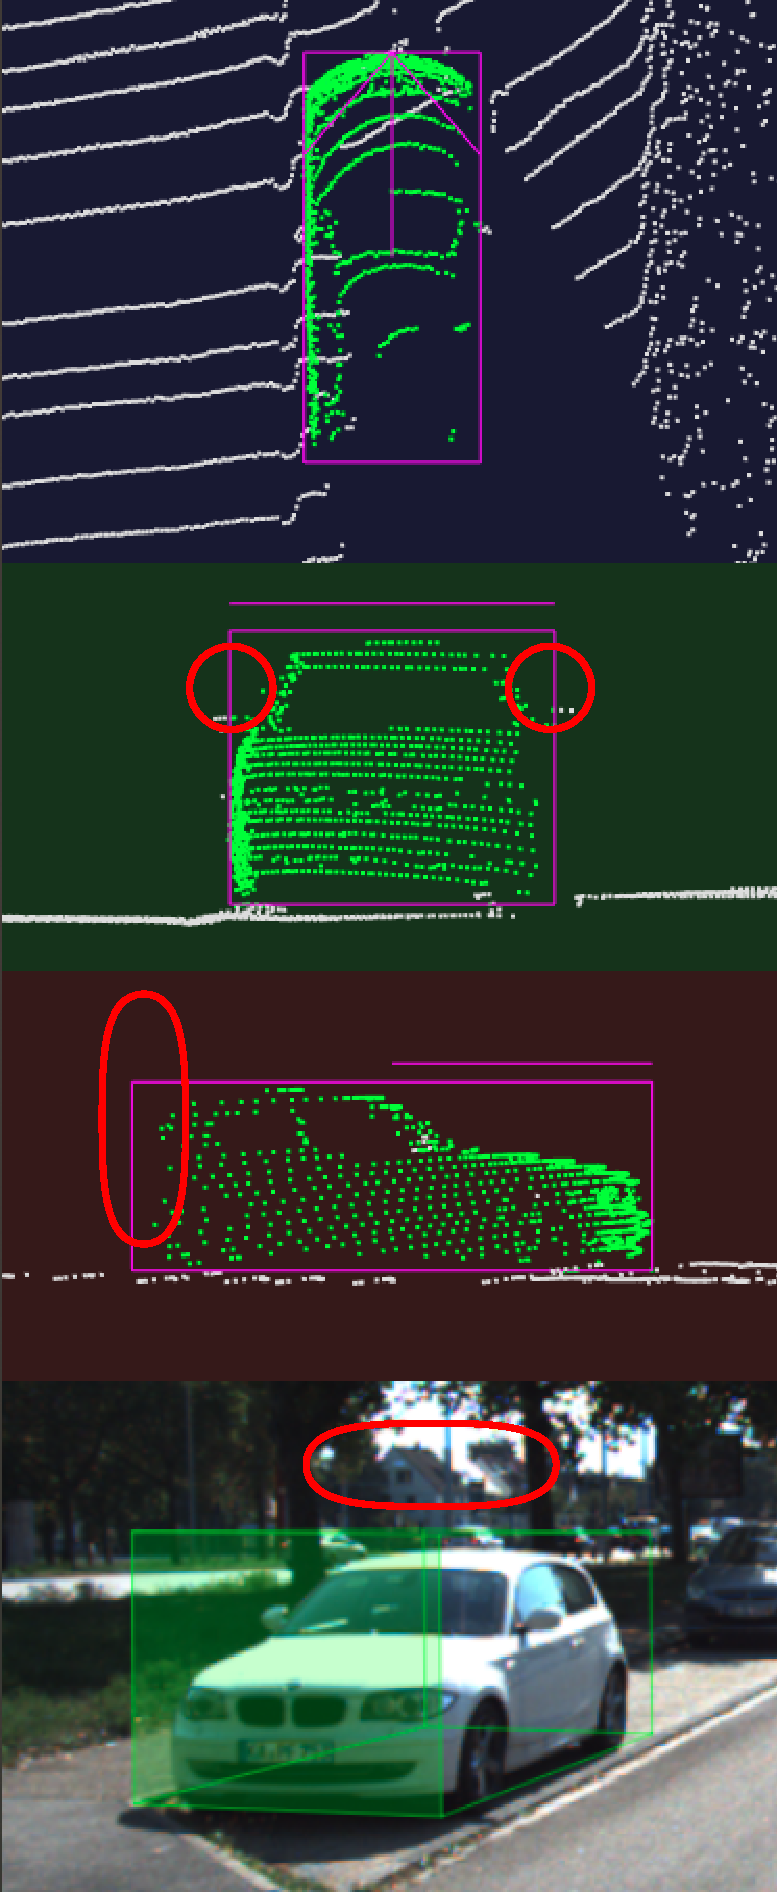
\includegraphics[scale=0.2]{./figures/annocheck-0}
	\end{subfigure}
	~
	\begin{subfigure}{0.3\linewidth}
		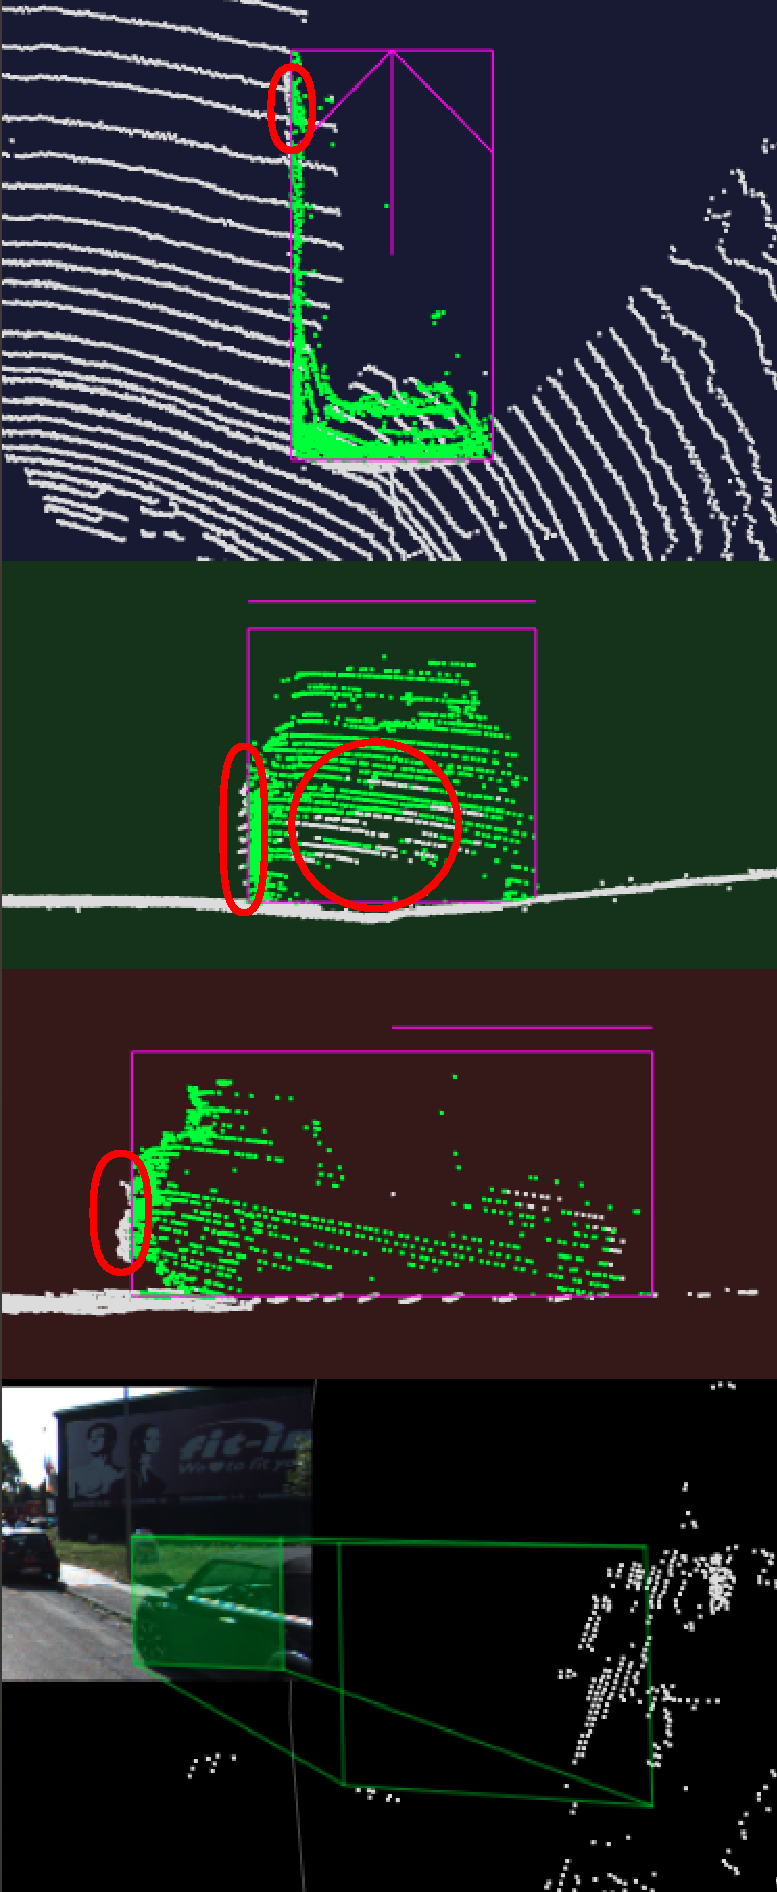
\includegraphics[scale=0.2]{./figures/annocheck-1}
	\end{subfigure}
	~
	\begin{subfigure}{0.3\linewidth}
		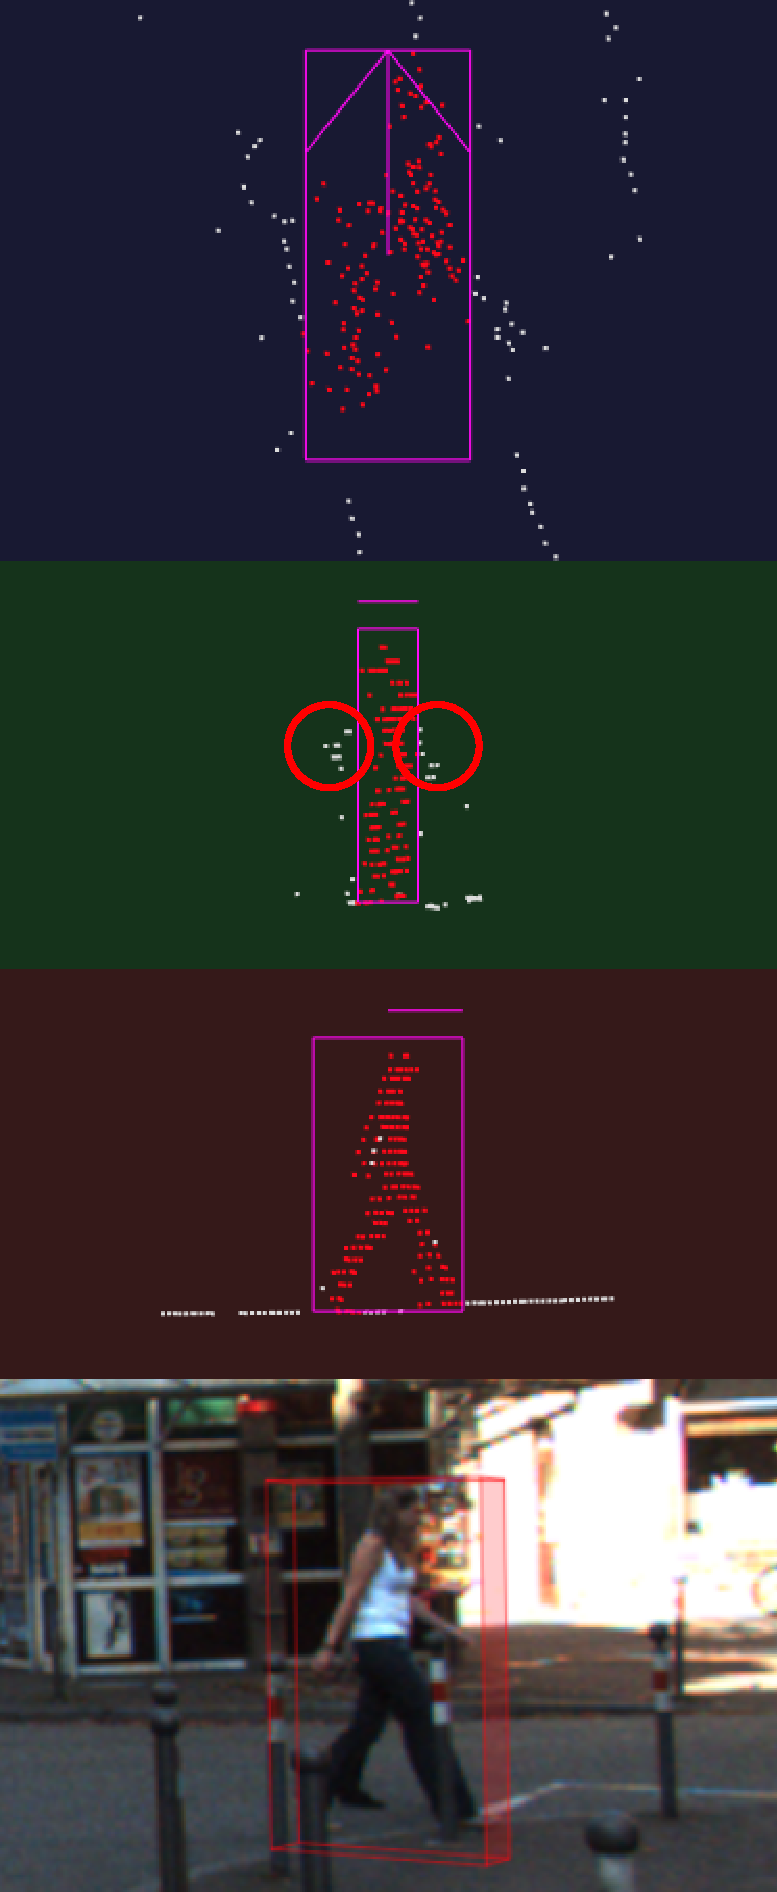
\includegraphics[scale=0.2]{./figures/annocheck-2}
	\end{subfigure}
	
	\caption{Checking inaccuracies in KITTI 3D object detection data set}
	\label{fig:annocheck}
\end{figure}


\subsection{Object Annotating}

Annotation efficiency can be measured by annotation time and accuracy\cite{pointatme} \cite{Zimmer20193DBA}. The time shall be minimized and accuracy maximized. \cite{Zimmer20193DBA} counts interpolated annotations in so the time per object is extremely small, for fairness we use \cite{pointatme} as the baseline to compare our platform with.

As described in \cite{pointatme} and also indicated in previous section, the original KITTI labels are not suited as ground truth for our benchmarks. So we carefully annotated some scenes and use the result as ground truth, 3 users are employed to annotate the same set of data, with a few hours of practicing beforehand. We choose the same scene as used in \cite{pointatme}. For ground truth annotation the average time used per object is less than 20 seconds.

For accuracy evaluation we follow the criteria  described in \cite{pointatme}, all points belonging to an object should be inside the bounding box and all points not belonging to it should be outside.
The test result is show in Table~\ref{tab:annotation-evaluation}.
\begin{table}[h]
	\centering
	\caption{Results compared with baseline}
	\label{tab:annotation-evaluation}
	\begin{tabular}{|l|c|c|c|c||c|c|c|c|}
		\hline
		\textbf{Method} & \textbf{Ours} & \textbf{PointAtME\cite{pointatme}} \\
		\hline
		\hline
		Time/Object (sec.) & 24 $\pm$ 6 & 55.2 $\pm$ 12.1\\
		\hline
		Undo/Object & - & 0.42 $\pm$ 0.43\\
		\hline
		Errors (Points/Object) & $<$1 & 28.7 $\pm$ 5.1\\
		\hline
		FP ratio / Object & - & 7.16\%\\
		\hline
		FN ratio / Object & - & 3.27\%\\
		\hline
	\end{tabular}
\end{table}


\subsection{Annotation transfer}
For annotation transfer we evaluate the accuracy. We  transfer annotations between frames that have 0.5 to 2.5 second difference in time, with our self-collected data set. The result is shown in Table~\ref{tab:transfer-evaluation}.



\begin{table}[h]
	\centering
	\caption{Accuracy of transfer annotations}
	\label{tab:transfer-evaluation}
	\begin{tabular}{|c|r|c|c|c|c|c|}
		\hline
		 & \textbf{Obj Type} & \textbf{Ref. Obj.}&\textbf{0.5s} & \textbf{1s} & \textbf{1.5s}& \textbf{2.5s} \\
		\hline
		\hline
		 1 & Car &-/1958& 15/1372 & 25/910 & 19/658 &  1/388\\
		\hline
  		 2 & Rider &-/329& 0/240 & 0/190 & 0149/658 &  0/94\\
		\hline
  		 3 & Bus &-/2327& 5/1208 & 3/656 & 1/396 &  0/244\\
\hline
	\end{tabular}

\begin{tabular}{p{\linewidth}}
	The content is Error/Total points. `Ref. Obj.` means reference object (i.e. manually annotated object)
\end{tabular}


\end{table}


\section{CONCLUSIONS}
\label{conclusions}

We introduced a novel 3D object annotation platform, focusing on visualization, operations and assisting algorithms. We demonstrated with tests that our platform can improve annotation accuracy with greater efficiency compared to other tools. The future direction will be to integrate more algorithms, for example, to integrate object tracking algorithm to work with our novel annotation transfer method to make our platform more efficient.



\addtolength{\textheight}{-12cm}   % This command serves to balance the column lengths
                                  % on the last page of the document manually. It shortens
                                  % the textheight of the last page by a suitable amount.
                                  % This command does not take effect until the next page
                                  % so it should come on the page before the last. Make
                                  % sure that you do not shorten the textheight too much.

%%%%%%%%%%%%%%%%%%%%%%%%%%%%%%%%%%%%%%%%%%%%%%%%%%%%%%%%%%%%%%%%%%%%%%%%%%%%%%%%



%%%%%%%%%%%%%%%%%%%%%%%%%%%%%%%%%%%%%%%%%%%%%%%%%%%%%%%%%%%%%%%%%%%%%%%%%%%%%%%%



%%%%%%%%%%%%%%%%%%%%%%%%%%%%%%%%%%%%%%%%%%%%%%%%%%%%%%%%%%%%%%%%%%%%%%%%%%%%%%%%
\begin{comment}


\section*{APPENDIX}

\subsection{Raw data orgnization}
In server, the raw data is organized by scenes, the directory structure is as in Fig.~\ref{fig:data-dir}.

\begin{figure}

	\dirtree{%
		.1 data.
		.2 scene1.
		.3 lidar.
		.4 frame0000.pcd.
		.4 ....
		.3 image.
		.4 left-camera.
		.5 frame0000.png.
		.5 ....
		.4 front.
		.5 frame0000.png.
		.5 ....
		.4 ....
		.3 calib.
		.4 left-camera.json.
		.4 front.json.
		.4 ....
		.3 label.
		.5 frame0000.json.
		.5 ....
		.2 scene2.
		.3 ....
		.2 ....
	}
	\caption{Raw data organization. The `label` folder is used to store annotation result. the `calib` folder stores lidar-camera calibration parameters, which is optional but requrired for 3d-2d fusion features. We list 3 cameras as an example, more cameras are also supported.}
	\label{fig:data-dir}
\end{figure}


\subsection{Operation summary}
\label{app:operations}
Table~\ref{table:keyboard_mainview} shows operations applicable in main view, Table~\ref{table:keyboard_subview} show operations applicable in side sub-views.

\begin{table}[h]
	\caption{Operations on main-view}
	\label{table:keyboard_mainview}
	\begin{center}
		\begin{tabular}{|c|l|}
			\hline
			\textbf{Key} & \textbf{Function}\\
			\hline
			1 & select previous object\\
			\hline
			2 & select next object\\
			\hline
			3 & previous frame\\
			\hline
			4 & next frame\\
			\hline
			r & rotate counterclockwise(yaw)\\
			\hline
			f & rotate clockwise(yaw)\\
			\hline
			t & reset box\\
			\hline
			g & reverse direction (yaw angle)\\
			\hline
			v & switch editing mode(Fig.~\ref{fig:box-mouse-edit})\\
			\hline
			Ctrl+s & save\\
			\hline
			Ctrl+c & copy reference box (\ref{semi-auto-anno})\\
			\hline
			Ctrl+z & undo\\
			\hline
			Ctrl+y & redo\\
			\hline
			Left drag & rotate view\\
			\hline
			Right drag & pan view\\
			\hline
			Wheel up & zoom in\\
			\hline
			Wheel down & zoom out\\
			\hline
			Ctrl+Left Drag (on main view)& mark points\\
			\hline
			Ctrl+Left click (on photo context)& draw polygon\\
			\hline
		\end{tabular}
	\end{center}
\end{table}


\begin{table}[h]
	\caption{Operations on sub-views}
	\label{table:keyboard_subview}
	\begin{center}
		\begin{tabular}{|c|l|c|l|}
			\hline
			\textbf{Key} & \textbf{Function}\\			
			\hline
			a & move left\\
			\hline
			s & move down\\
			\hline
			d & move right\\
			\hline
			w & move up\\
			\hline
			q & rotate left\\
			\hline
			e & rotate right\\
			\hline
			q & rotate left\\
			\hline
			e & rotate right\\
			\hline				
			Ctrl-q & rotate left with boundary aware\\
			\hline
			Ctrl-e & rotate right with boundary aware\\
			\hline
			Drag box border/corner & resizing box\\
			\hline
			Drag direction line & rotate box\\
			\hline
			Drag box border/corner with Ctrl hold & resizing box with auto-shrink\\
			\hline
			Drag direction line with Ctrl hold& rotate box with boundary aware\\
			\hline
			Drag box center & move box\\
			\hline
			Double click box border/corner & auto-shrinking\\
			\hline
			Double click box center & auto-shrinking all borders\\
			\hline
			Double click direction line& rotate upside-down (180 degree)\\
			\hline
		\end{tabular}
	
		 {\raggedright Note that all operation effects are relative to current sub-view.\par}
		 
	\end{center}
\end{table}
\section*{ACKNOWLEDGMENT}


\end{comment}

%%%%%%%%%%%%%%%%%%%%%%%%%%%%%%%%%%%%%%%%%%%%%%%%%%%%%%%%%%%%%%%%%%%%%%%%%%%%%%%%


\bibliographystyle{IEEEtran}
\bibliography{MyReference}
\end{document}
